\documentclass[../main.tex]{subfiles}
\graphicspath{{\subfix{../images/}}}

\begin{document}

    \chapter{Tecnologie di Background}
	
    	\section{Cloud Provider: \emph{AWS}}
    	
    	    \begin{figure}[h]
    			\centering
    			
\includegraphics[width=0.2\textwidth]{aws_logo}
    			\caption{Logo Amazon Web Services - \textbf{Source}: AWS}
    			\label{fig:aws_logo}
    	    \end{figure}
    	
    	    Per implementare il processo high-level descritto nel \hyperref[sec:devops_process]{capitolo precedente}, ci si è forniti del provider di servizi cloud \emph{Amazon Web Services}, scelto per la sua completezza di servizi offerti e competitività sul mercato.
    	    
    	    \begin{figure}[H]
    			\centering
    			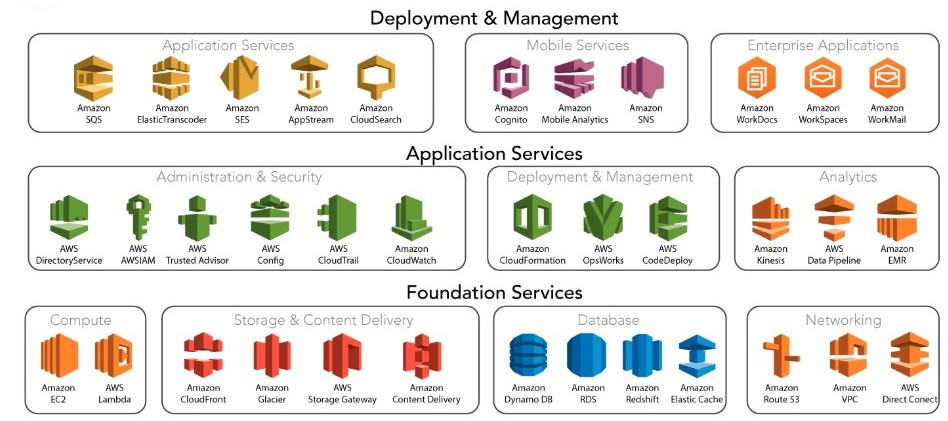
\includegraphics[width=\textwidth]{aws_services}
    			\caption{Servizi AWS (principali) - \textbf{Source:} AWS}
    			\label{fig:aws_services}
    	    \end{figure}
    	    
    	    I servizi che offre AWS (figura \ref{fig:aws_services}) si dividono sui 3 livelli della piramide cloud:
    	    \begin{itemize}
    	        \item \textbf{Infrastructure-as-a-Service}
    	        \begin{itemize}
    	            \item \emph{Networking}: Virtual Private Cloud (VPC), Route 53 (DNS);
    	            \item \emph{VM}: Elastic Compute Cloud (EC2);
    	            \item \emph{Storage}: Elastic Block Storage (EBS);
    	        \end{itemize}
    	        \item \textbf{Platform-as-a-Service}:
    	        \begin{itemize}
    	            \item \emph{Database}: DynamoDB, Relational Database Service (RDS);
    	            \item \emph{Mobile}: Cognito, Mobile Analytics;
    	            \item \emph{Messaging}: Simple Queue Service (SQS), Simple Notification Service (SNS), Simple Email Service (SES);
    	        \end{itemize}
    	        \item \textbf{Software-as-a-Service}:
    	        \begin{itemize}
    	            \item \emph{Identity}: Identity and Access Management (IAM), Directory Service (DS);
    	            \item \emph{Monitoring}: CloudWatch, CloudTrail, X-Ray;
    	            \item \emph{Storage}: CloudFront, Simple Storage Service (S3).
    	        \end{itemize}
    	    \end{itemize}
    	    
    	    Esistono molti altri servizi che non descriveremo ne utilizzeremo in questo progetto, questo fa intuire la vastità dell'offerta di \emph{AWS} e come possa risultare estremamente flessibile in base alle esigenze. Nel nostro caso utilizzeremo i seguenti servizi per configurare la piattaforma che gestirà il processo \emph{DevOps}:
    	    \begin{itemize}
    	        \item Networking basato su \textbf{VPC} e \textbf{Route 53} (reti private e DNS privato gestito);
    	        \item Macchine Virtuali basate su \textbf{EC2} con storage \textbf{EBS} di tipologia GP2 (General Purpose);
    	        \item Servizio VPN basato su \textbf{AWS Client VPN} (OpenVPN Server) per accedere alle risorse private;
    	        \item Load Balancing dei servizi basato su \textbf{Elastic Load Balancer} (ELB), usato in varianti \emph{Classic} e \emph{Application} in base all'applicativo;
    	        \item Docker Registry basato su \textbf{Elastic Container Registry} (ECR).
    	        \end{itemize}
    	
    	\section{Infrastructure-as-Code: \emph{Terraform}}
    	
    	    Per creare l'infrastruttura sfruttando il paradigma di \emph{Infrastructure-as-Code} è stato scelto l'utilizzo di \textbf{Terraform}\cite{terraform}, il tool \emph{de facto} standard in ambienti multicloud che vogliono evitare il \emph{vendor lock} delle proprie risorse.
    	    
    	    \begin{figure}[H]
    			\centering
    			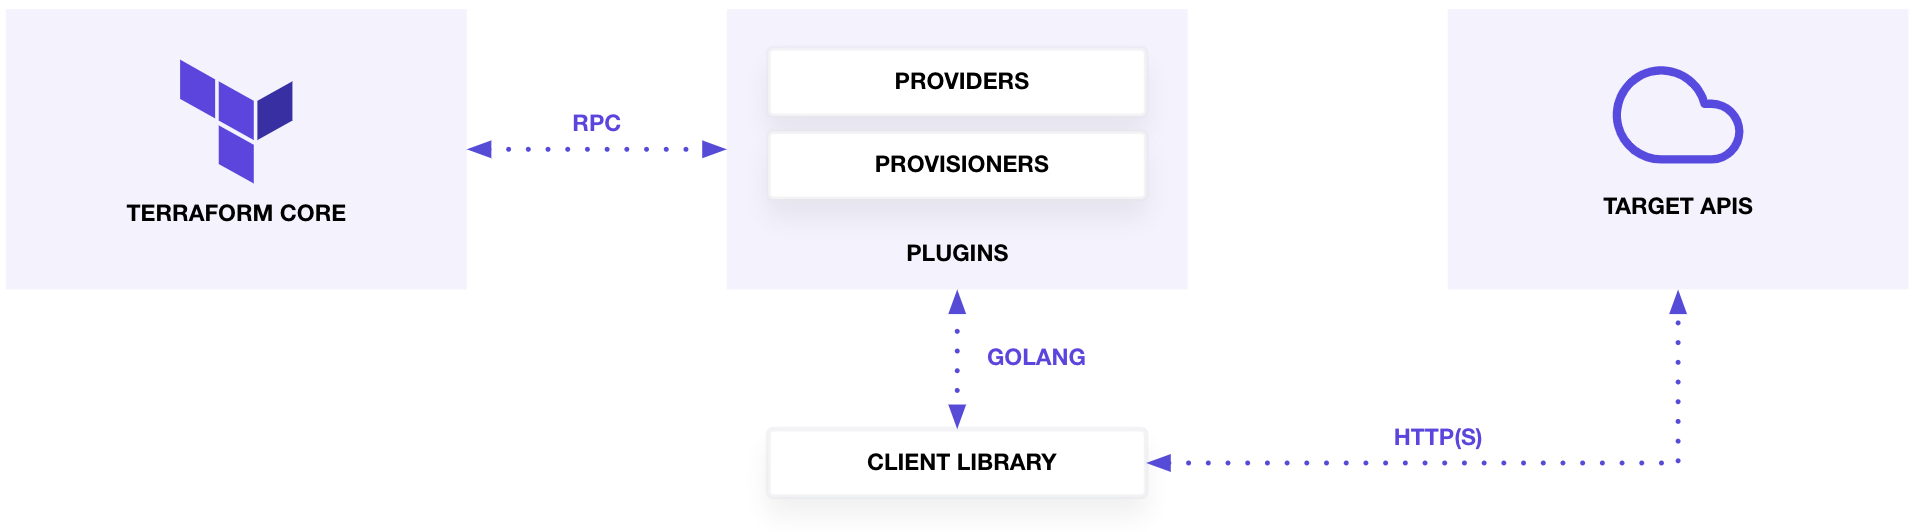
\includegraphics[width=\textwidth]{terraform_schema}
    			\caption{Terraform - Schema Funzionamento - \textbf{Source:} HashiCorp}
    			\label{fig:terraform_schema}
    	    \end{figure}
    	    
    	    Sviluppato da \textbf{HashiCorp} in \emph{Go}, si presenta come una \emph{CLI} ed un linguaggio dedicato chiamato \textbf{HCL} (\emph{HashiCorp Configuration Language}), mediante il quale si esprime lo stato voluto delle risorse (dichiarativo) che poi il tool convertirà in azioni di creazione, modifica o cancellazione nell'ambiente cloud scelto.\\*
    	    
    	    Grazie alla sua struttura è possibile modularizzare e parametrizzare il codice, in modo da adattarsi a vari tipi di deployment e generalizzare le implementazioni, esattamente come si farebbe con un linguaggio comune (imperativo, funzionale, OO). Terraform, al momento di applicare le modifiche, \textbf{interroga} prima la cloud platform target sullo stato attuale delle risorse, adattando così il suo stato interno (che può essere mantenuto anche in remoto) e creando la \textbf{lista delle modifiche} da applicare per arrivare allo stato desiderato. Questa tecnica inoltre rileva e tiene conto delle \textbf{dipendenze tra le risorse} mediante la creazione di un grafo dedicato, ad esempio un entry DNS necessiterà di un target specifico, che dovrà essere quindi creato prima della entry stessa.\\*
    	    
    	    Un lato negativo nell'utilizzo di Terraform è la \textbf{non possibilità di effettuare dei rollback} mirati una volta che le modifiche sono state applicate. Per fare ciò servirà infatti fare un "revert" del codice modificato, e poi applicare di nuovo le modifiche, ma non vi è una funzione dedicata a riguardo.
    	    
    	    \subsection{Esempio: Creazione di una VM}
    	    
    	        Prenderemo come esempio la creazione di una istanza server virtuale in ambiente \textbf{AWS}, quindi la risorsa sarà di tipo \textbf{EC2} e necessiterà di diversi elementi di contorno per essere definita. In primis Terraform necessita di definire un \textbf{\emph{provider}}, ovvero un "driver" che gli permetta di interfacciarsi con una cloud platform, in questo caso AWS, in un file nominato \verb|main.tf|:
    	        \begin{lstlisting}
provider "aws" {
    region = "eu-west-1"
}
    	        \end{lstlisting}
    	        
    	        Successivamente definiremo subito sotto la nostra istanza sfruttando la tipologia di risorsa chiamata \verb|aws_instance| come descritta nella documentazione ufficiale:
    	            	        \begin{lstlisting}
resource "aws_instance" "example" {
    ami           = "ami-something"
    instance_type = "t3.micro"
}
    	        \end{lstlisting}
    	        
    	        In seguito bisognerà inizializzare Terraform mediante il comando \verb|init| che permette di creare il "backend" (lo stato) del sistema e di scaricare tutte le dipendenze di cui necessita (providers, definizioni):
    	        \begin{lstlisting}[language=bash]
$ terraform init

Initializing the backend...

Initializing provider plugins...
- Checking for available provider plugins...
- Downloading plugin for provider "aws"

(...)

* provider.aws: version = "~> 2.10"

Terraform has been successfully initialized!
                \end{lstlisting}
                
                In seguito si potranno visualizzare ed applicare le modifiche usando i comandi \verb|plan| ed \verb|apply|, il primo della quale crea un report delle modifiche da applicare, mentre il secondo oltre a crearlo permette anche di applicare le modifiche listate in quel report:
    	        \begin{lstlisting}[language=bash]
$ terraform apply

(...)

Terraform will perform the following actions:  
    # aws_instance.example will be created
    + resource "aws_instance" "example" {
        + ami                          = "ami-something"
        + arn                          = (known after apply)
        + associate_public_ip_address  = (known after apply)
        + availability_zone            = (known after apply)
        + cpu_core_count               = (known after apply)
        + cpu_threads_per_core         = (known after apply)
        + get_password_data            = false
        + host_id                      = (known after apply)
        + id                           = (known after apply)
        + instance_state               = (known after apply)
        + instance_type                = "t3.micro"
        + ipv6_address_count           = (known after apply)
        + ipv6_addresses               = (known after apply)
        + key_name                     = (known after apply)
        (...)
  }
  
  Plan: 1 to add, 0 to change, 0 to destroy.
  
  Do you want to perform these actions?
  Terraform will perform the actions described above.
  Only 'yes' will be accepted to approve.
  
  Enter a value:
                \end{lstlisting}
    	
    	\section{Configuration-as-Code: \emph{Ansible}}
    	
    	    Per la gestione della configurazione dei servizi all'interno dell'infrastruttura creata, è stato scelto l'utilizzo di \textbf{Red Hat Ansible}\cite{ansible}, uno dei tool di configuration più utilizzati al mondo assieme ai competitor \emph{Chef} e \emph{Puppet}.
    	    
    	    \begin{figure}[H]
    			\centering
    			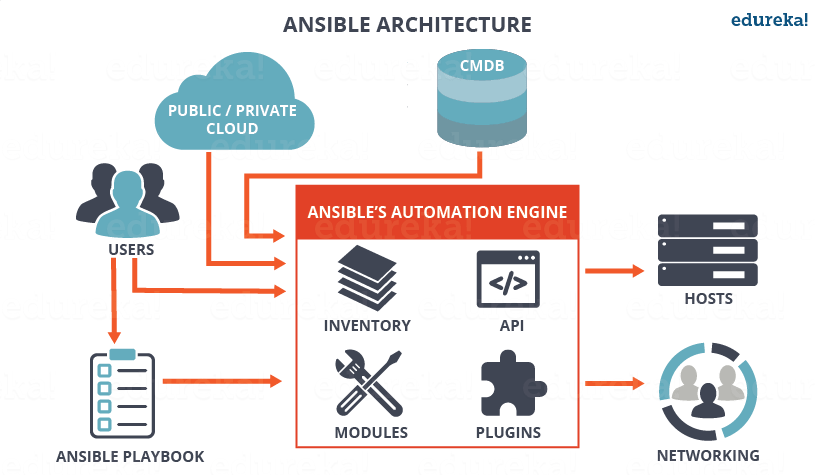
\includegraphics[width=0.8\textwidth]{ansible_schema}
    			\caption{Ansible - Schema Funzionamento - \textbf{Source:} Edureka!}
    			\label{fig:ansible_schema}
    	    \end{figure}
    	    
    	    Ansible permette di gestire intere flotte di macchine mantenendo sempre lo stato delle cose ed uno stato desiderato, soppiantando così la vecchia pratica degli script "usa e getta" utilizzati in ambito sistemistico. Ansible sfrutta una sintassi semplice scritta in \textbf{YAML} (\emph{YAML Ain't a Markup Language}) mediante ciò che viene definito un \textbf{playbook}, che definisce la lista ordinata dei task da effettuare per eseguire una determinata azione.\\*
    	    
    	    Mediante la creazione di \textbf{roles} si possono generalizzare i \emph{playbook} creati, che possono poi essere eseguiti ad un livello superiore di astrazione. Per gestire le variabili di processo interne Ansible sfrutta i \textbf{facts}, richiamabili da qualsiasi punto dei \emph{playbook} e dove si possono memorizzare dati anche lungo il corso di un processo. Infine, per definire i suoi target di lavoro (macchine locali o remote), viene creato un \textbf{inventory} in modo statico o dinamico, dove si descrive il target (IP, porta) e il metodo con cui collegarsi ad esso.
    	    
    	    \subsection{Esempio: installazione di Apache Httpd}
    	    
    	        Per definire un esempio di utilizzo degli \emph{Ansible Playbooks}, illustreremo l'installazione del server Apache Httpd su un ipotetico host remoto mediante accesso SSH. In primis si necessita definire il file dell'\emph{inventory} di Ansible, contenente il nome degli host (friendly), il loro IP e la porta a cui connettersi:
    	        \begin{lstlisting}[language={Ini}]
[group1]
host1 ansible_host=192.168.100.2 ansible_ssh_port=22
[group2]
host2 ansible_host=192.168.100.3 ansible_ssh_port=22
    	        \end{lstlisting}
    	        
    	        In seguito si scrive il \emph{playbook} mediante codice \textbf{YAML}, definendo le azioni da fare in base al nome dato agli host nell'\emph{inventory}. Tali azioni sono definite dal framework di Ansible stesso o mediante plugins esterni, possono definire condizioni, variabili e possono essere applicate più volte senza preoccuparsi di conflitti (Ansible controlla preventivamente lo stato):
    	        \begin{lstlisting}[language=yaml]
---
- hosts: group1, group2
  tasks:
  - name: Install Apache Httpd
    yum:
      name: httpd
      state: present
    when: ansible_system_vendor == 'AWS' and ansible_os_family == 'RedHat'
    	        \end{lstlisting}
    	
    	        Per avviare un Ansible Playbook basterà richiamare la CLI mediante un terminale (shell) con la seguente sintassi:
    	        \begin{lstlisting}[language=bash]
$ ansible-playbook -i hosts.ini playbook.yaml
    	        \end{lstlisting}
    	        dove \verb|-i| indica l'\emph{inventory} creato precedentemente e \verb|playbook.yaml| il file di \emph{playbook} creato con le nostre azioni da eseguire. Durante il processo potremo visionare le singole azioni che vengono compiute sui singoli hosts definiti, e otterremo alla fine un report con eventuali errori avvenuti durante il processo.
    	
    	\section{Container Engine: \emph{Docker}}
    	    
    	    Come precedentemente descritto nel \hyperref[sec:cloud_containers]{capitolo dedicato al Cloud}, in un processo \emph{DevOps} risulta importante mantenere consistente l'ambiente di sviluppo, testing e deployment del software. Per fare ciò vengono sfruttati i \textbf{Containers} e più precisamente l'engine di \textbf{Docker}\cite{docker}, uno dei più diffusi al mondo e semplici da utilizzare.
    	    
    	    \begin{figure}[H]
    			\centering
    			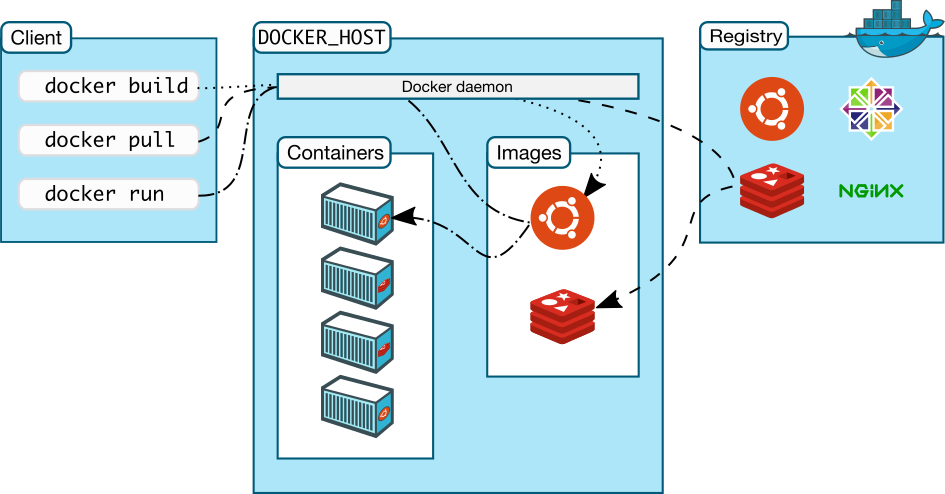
\includegraphics[width=0.8\textwidth]{docker_arch}
    			\caption{Docker - Schema Funzionamento - \textbf{Source:} Docker}
    			\label{fig:docker_arch}
    	    \end{figure}
    	    
    	    Docker si compone di un \textbf{\emph{daemon}} (processo) che gestisce il \emph{container runtime} sottostante (basato su \emph{runC}) e che offre un accesso facilitato ai container mediante delle API, ed un \textbf{client} usabile via CLI oppure interfaccia grafica (in base alle implementazioni). Oltre a gestire il runtime, Docker fornisce facile accesso alla gestione delle \textbf{immagini} dei container stessi, scaricabili online o compilabili localmente a partire da un \textbf{Dockerfile}, e fornisce inoltre un livello di astrazione sulla gestione dei \textbf{volumi} agganciabili ai container in esecuzione (mediante \emph{binding} con una cartella locale, o mediante volumi interamente gestiti).\\*
    	    
    	    Oltre all'utilizzo per distribuire gli artefatti applicativi, nel progetto verrà utilizzato Docker per eseguire l'installazione e la configurazione facilitata degli strumenti da utilizzare sulle macchine virtuali, evitando tediosi processi di installazione e velocizzando futuri aggiornamenti grazie alla mera sostituzione della immagine di base.
    	    
    	    \subsection{Esempio: applicazione Java}
    	    
    	        Avendo un applicativo Java sotto forma di file \verb|.jar| eseguibile, possiamo definire il \verb|Dockerfile| che contenga il runtime della JVM, le dipendenze necessarie e che permetta di eseguire l'applicazione mediante l'uso di un container engine:
    	        \begin{lstlisting}[language=docker]
FROM openjdk:8-jdk-alpine # Base image
WORKDIR /usr/app # Working directory
COPY ./app.jar app.jar # Copy file from local to container
ENTRYPOINT ["java","-jar","/usr/app/app.jar"] # Run the app
    	        \end{lstlisting}
    	        
    	        Mediante questo Dockerfile, a seguito della build con la CLI di \verb|docker| e i comandi \verb|build| e \verb|tag|, verrà creata una immagine basata sulla immagine pubblica \verb|openjdk:8-jdk-alpine| con il file \verb|app.jar| al suo interno che verrà avviato come processo java "controllato" dal container al momento della sua creazione.
    	        
\end{document}